\chapter{Основная часть}


\section{Настройка окружения}

Используя VirtualBox, развернём две виртуальные машины - с Kali Linux и Metasploitable.
Объединим их в одну сеть.

\begin{figure}[H]
	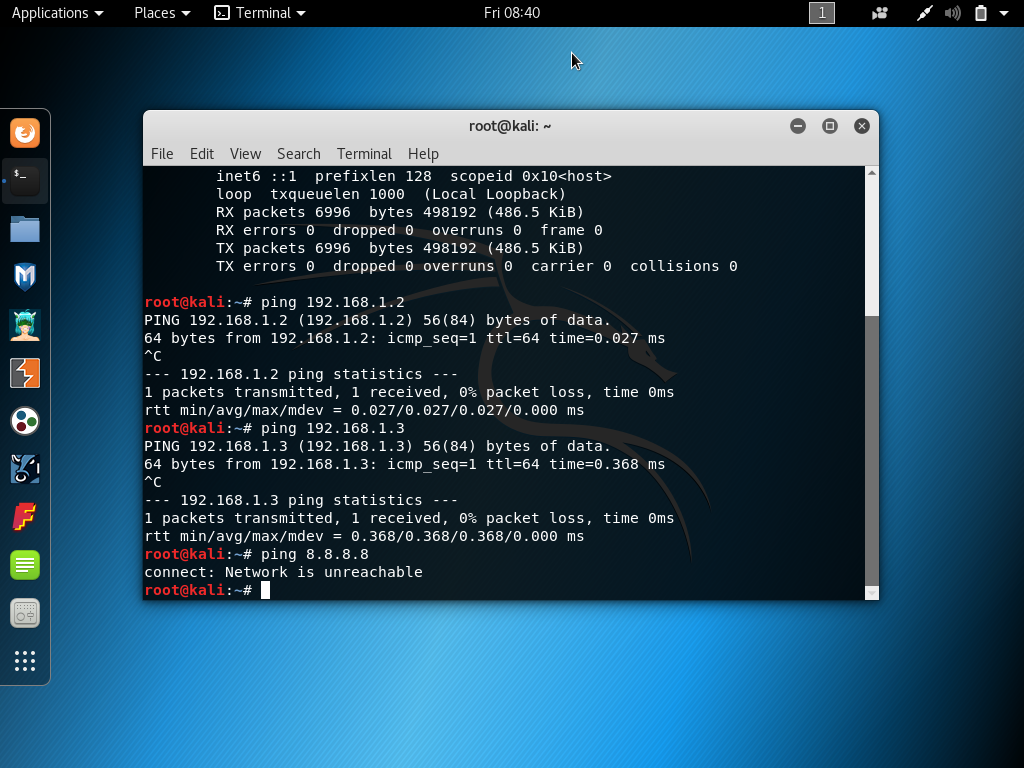
\includegraphics[width=\textwidth]{images/kali_ping.png}
\end{figure}

\begin{figure}[H]
	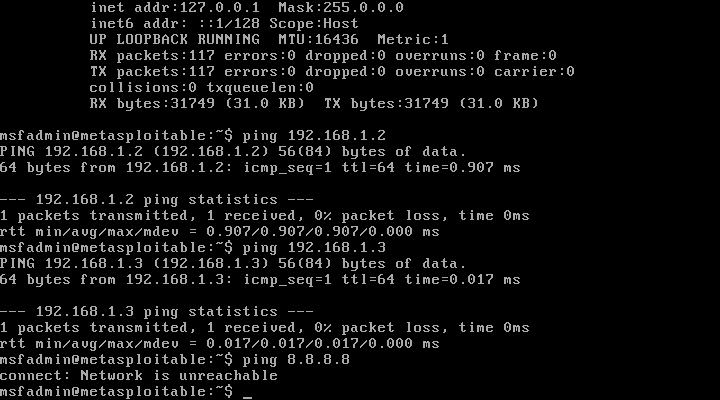
\includegraphics[width=\textwidth]{images/meta_ping.png}
\end{figure}

\section{Сканирование портов}

\begin{figure}[H]
	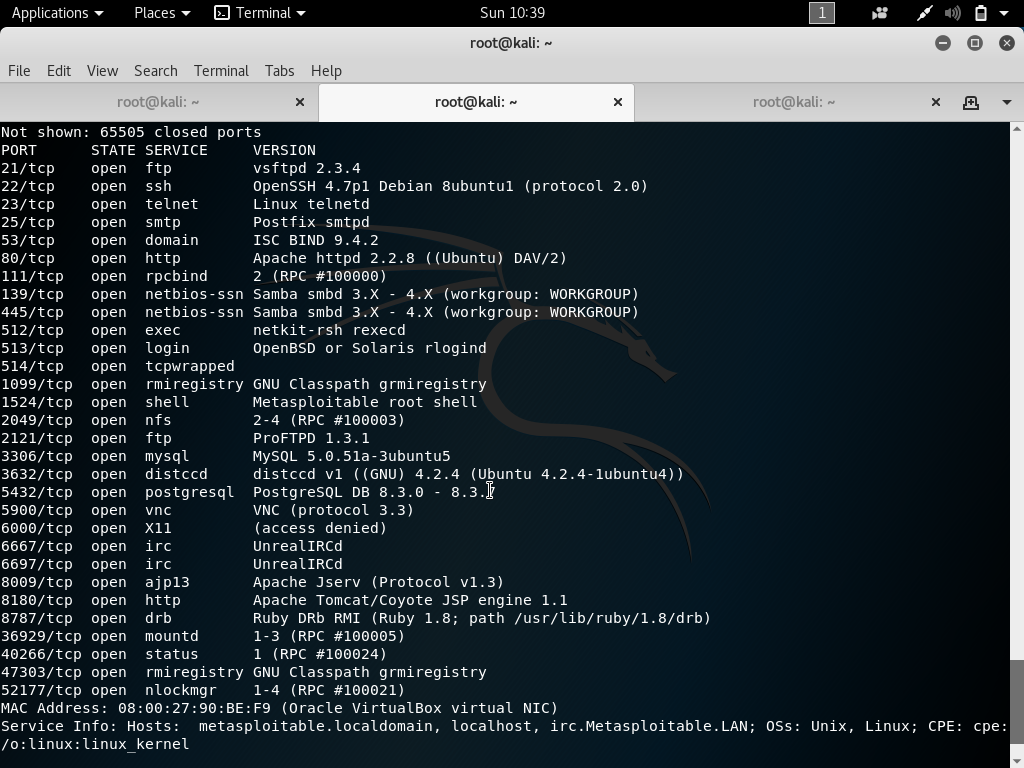
\includegraphics[width=\textwidth]{images/nmap.png}
\end{figure}


\section{Получение доступа}

\subsection{UnrealIRCd}

\begin{figure}[H]
	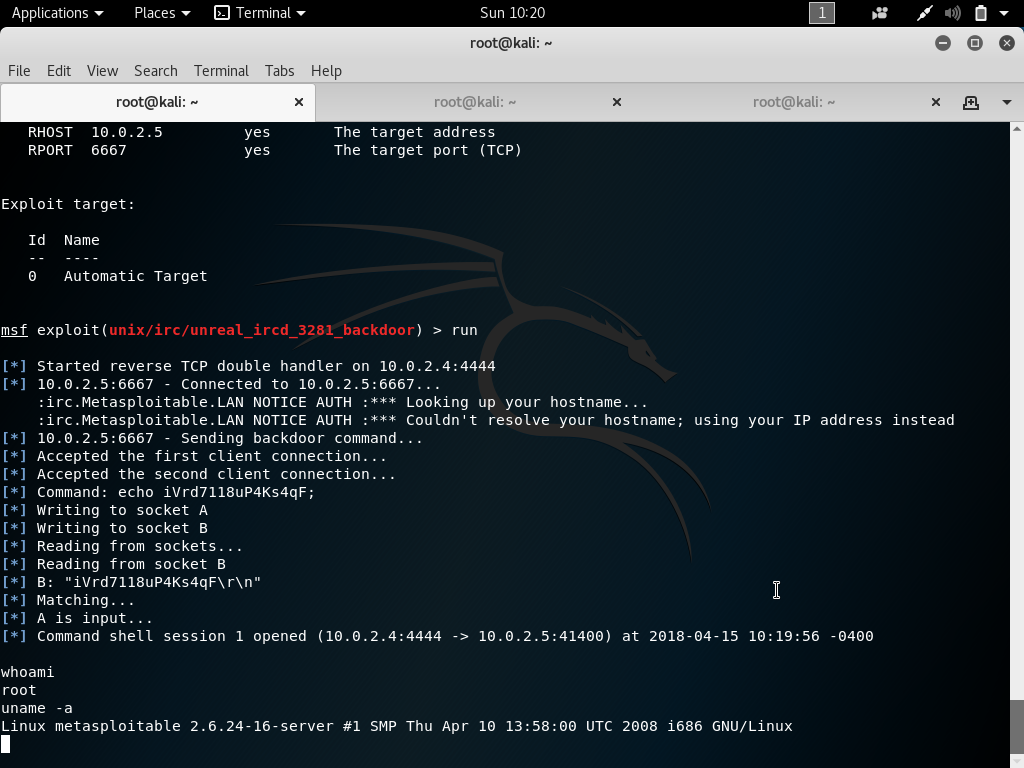
\includegraphics[width=\textwidth]{images/ircd.png}
\end{figure}

\subsection{Java RMI Server}

\begin{figure}[H]
	\includegraphics[width=\textwidth]{images/java_rmi.png}
\end{figure}

\subsection{NFS}

\begin{figure}[H]
	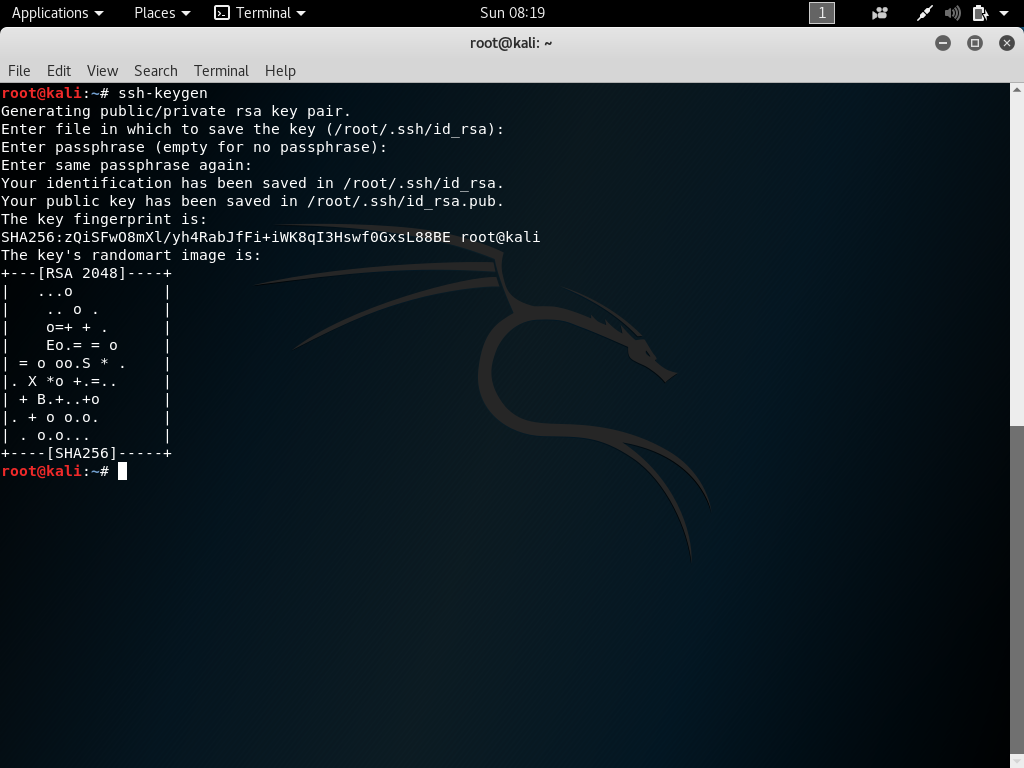
\includegraphics[width=\textwidth]{images/nfs1.png}
\end{figure}

\begin{figure}[H]
	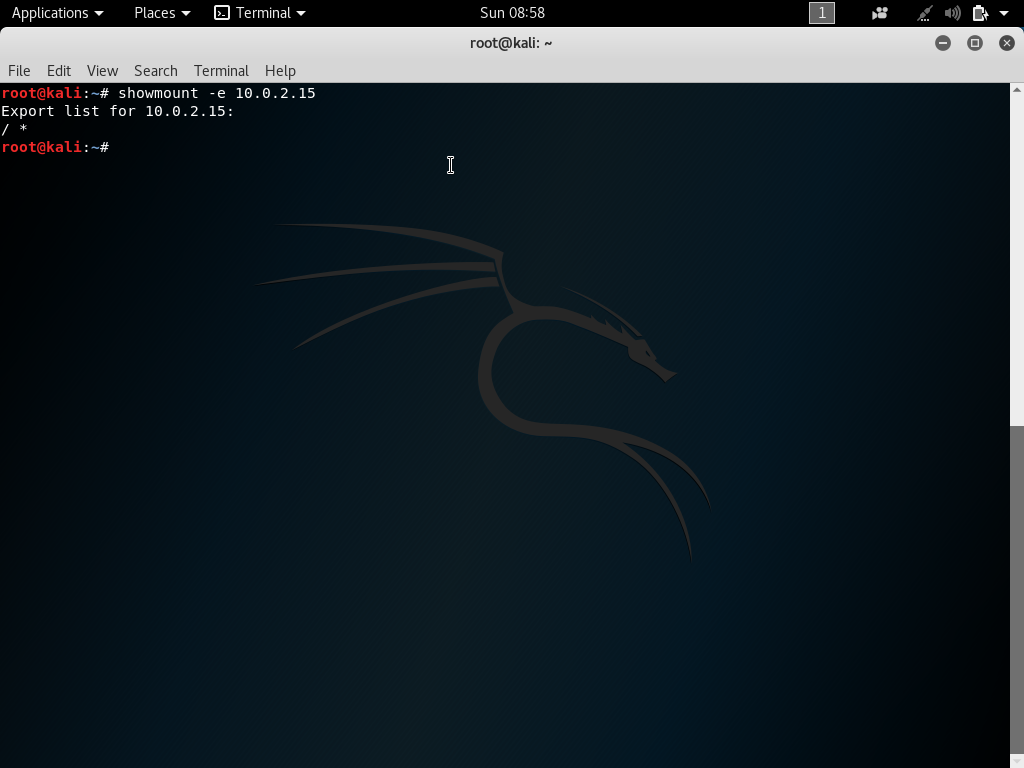
\includegraphics[width=\textwidth]{images/nfs2.png}
\end{figure}

\begin{figure}[H]
	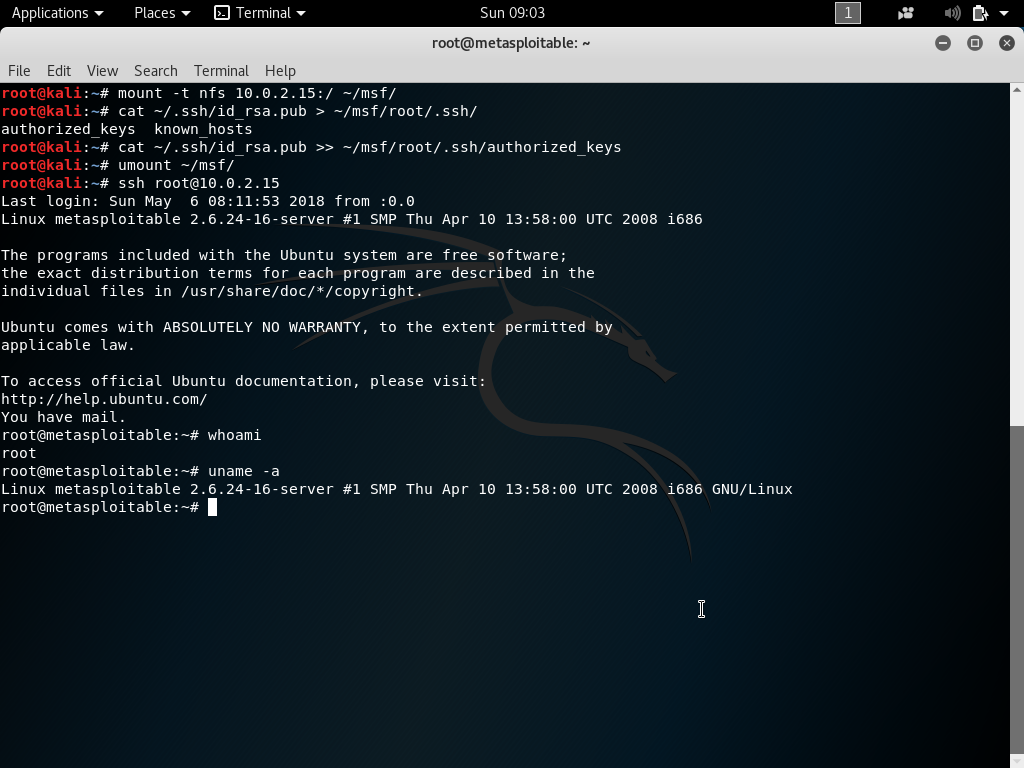
\includegraphics[width=\textwidth]{images/nfs3.png}
\end{figure}

\subsection{Port 1524}

\begin{figure}[H]
	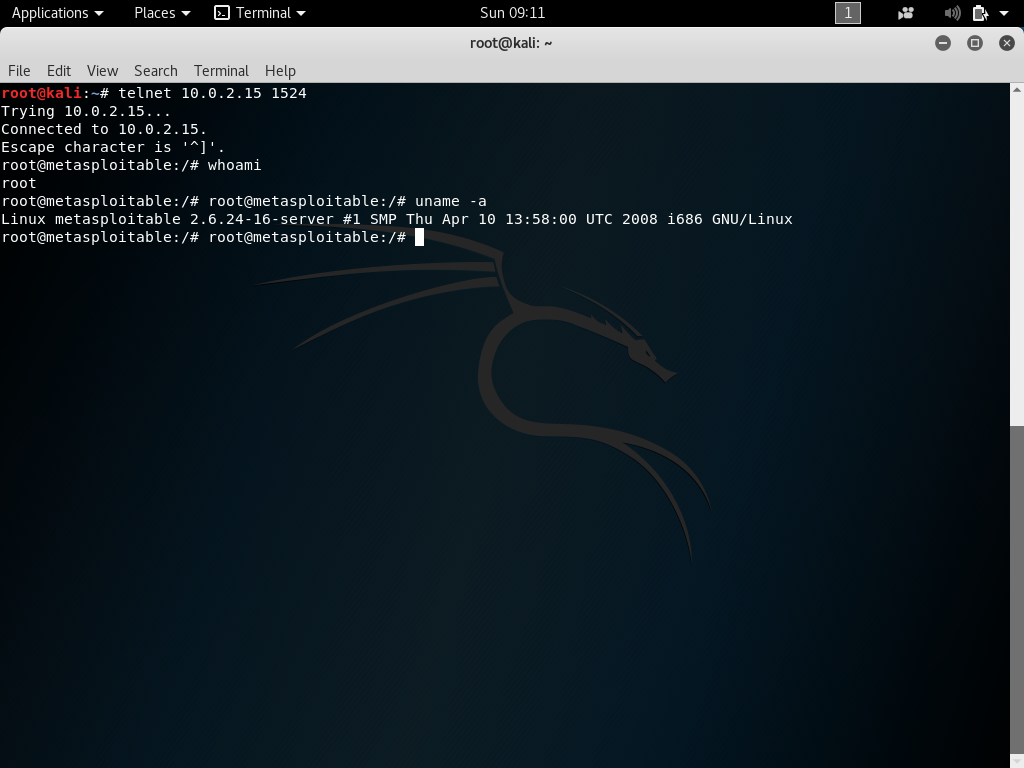
\includegraphics[width=\textwidth]{images/ingres.png}
\end{figure}

